\documentclass[../main.tex]
		
		\begin{document}
			\section{Connected Graphs}
	\begin{description}
		\item[Task:] Use the ideas above related to traversing parts of a graph in order to define a particularly important category of graphs.
		\item[Definition:] An undirected graph $(V, E)$ is called \underline{connected} if $\forall u, v \in V$ vertices, $\exists$ path in the graph from $u$ to $v$.
		\item[Examples:]
		\begin{enumerate}
			\item Is not connected as $d$ is not connected to any other vertex.
			\begin{figure}[h!]
				\centering
				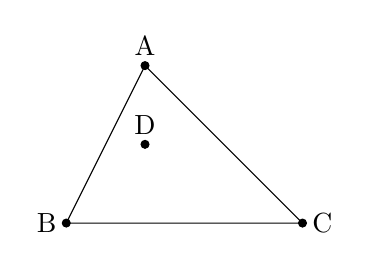
\begin{tikzpicture}
				\coordinate (A) at (0, 0);
				\coordinate (B) at (-1, -2);
				\coordinate (C) at (2, -2);
				\coordinate (D) at (0, -1);
				
				\draw (A) -- (B) -- (C) -- (A);
				\draw[fill=black] (A) circle[radius=0.5mm] node[above]{A};
				\draw[fill=black] (B) circle[radius=0.5mm] node[left]{B};
				\draw[fill=black] (C) circle[radius=0.5mm] node[right]{C};
				\draw[fill=black] (D) circle[radius=0.5mm] node[above]{D};
				\end{tikzpicture}
			\end{figure}
			\pagebreak
			\item Is connected. $\exists$ path between any two of the vertices.
			\begin{figure}[h!]
				\centering
				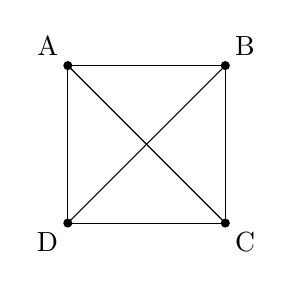
\begin{tikzpicture}
				\coordinate (A) at (-1, 1);
				\coordinate (B) at (1, 1);
				\coordinate (C) at (1, -1);
				\coordinate (D) at (-1, -1);
				
				\draw (A) -- (B) -- (C) -- (D) -- (A);
				\draw (A) -- (C);
				\draw (D) -- (B);
				
				\draw[fill=black] (A) circle[radius=0.5mm] node[above left]{A};
				\draw[fill=black] (B) circle[radius=0.5mm] node[above right]{B};
				\draw[fill=black] (C) circle[radius=0.5mm] node[below right]{C};
				\draw[fill=black] (D) circle[radius=0.5mm] node[below left]{D};
				\end{tikzpicture}
			\end{figure}
		\end{enumerate}
		\item[Theorem:] Let $(V, E)$ be a undirected graph, and let $u, v \in V. \exists$ path between $u$ and $v$ in the graph $\Leftrightarrow \exists$ walk in the graph between $u$ and $v$.
		\item[Proof:] $\Rightarrow$ trivial: A path is a walk. \\
		$\Leftarrow \exists$ walk between $u$ and $v$. Choose the walk of least length between $u$ and $v$, (\textbf{i.e.} $\nexists$ a walk of lower length than this one) and prove it is a path. Let this walk be $a_0 a_1 \dots a_n$ with $a_0 = u$ and $a_n = v$. Assume $\exists j, k$ with $a \leq j, k \leq n$ s.t. $j < k$ and $a_j = a_k$, but then $a_0 a_1 \dots a_j a_k+1 \dots a_n$ would be a walk from $u$ to $v$ of \underline{strictly smaller} length than $a_0 a_1 \dots a_n$. $\Rightarrow \Leftarrow$ as we chose $a_0 a_1 \dots a_n$ to be of minimal length $ \Rightarrow a_i \neq a_j \forall i, j$ s.t. $0 \leq i, j \leq n \Rightarrow a_0 a_1 \dots a_n$ is a path between $u$ and $v$.
		\item[qed]
		\item[Corollary:] An undirected grapg $(V, E)$ is connected $\Leftrightarrow \forall u, v \in V \exists$ walk in the graph between $u$ and $v$.
	\end{description}
	

\end{document}